0. \underline{Introducción}

0.1. En la presente exposición aplicamos los resultados de las
exposiciones precedentes al estudio del \underline{modelo de Néron}
(1.1) $A$ de un esquema abeliano $A_K$ definido sobre el cuerpo de
funciones $K$ del rasgo henseliano $S$. Veremos que las propiedades más
importantes del modelo de Néron pueden interpretarse mediante la acción
del grupo de monodromía local $I$ sobre el módulo de Tate
$T_\ell(A_K(\overline K))$ (donde $\ell$ es un número primo distinto de
$p$). Puesto que el dual de este último puede interpretarse como el grupo
de cohomología $\ell$-ádica $H^1(A_{\overline K},\mathbb Z_\ell)$, y
puesto que, para todo esquema proyectivo liso $X$ sobre $K$,
$H^1(X_{\overline K},\mathbb Z_\ell)$ se identifica con
$H^1(A_{\overline K},\mathbb Z_\ell)$, donde $A_{\overline K}$ es la
variedad de Albanese de $X_{\overline K}$, la presente exposición puede
considerarse también como un estudio detallado de los
\underline{fenómenos de monodromía local para la cohomología
$\ell$-ádica} $H^1$
(o, mejor aún, para el $H^1$ «motívico») \underline{de las variedades
proyectivas lisas sobre} $K$. Desde este punto de vista, parece claro
que los resultados principales de la presente exposición están
destinados a integrarse en una «teoría de Néron» para motivos de peso
arbitrario, es decir, para $H^i$ ($\ell$-ádico, de Rham, de Hodge,
etcétera) con $i$ arbitrario, de la cual apenas comenzamos ahora a
entrever algunos rasgos. (Véase [9] a este respecto y, más
particularmente, las Conjeturas 9.8 a 9.13 de Deligne en el informe
citado.)

0.2. El resultado más importante de la presente exposición es el
«\underline{teorema de reducción semiestable}» 3.6, que afirma que,
tras una extensión separable finita $K'$ de $K$, el modelo de Néron de
$A_{K'}$ posee una fibra especial cuya componente neutra es una
extensión de un esquema abeliano por un toro. Este resultado fue
conjeturado por J.-P. Serre en 1964, y el principio de la demostración
dada aquí\footnote{Se desarrolla en una carta del conferenciante a
J.-P. Serre fechada el 30 de octubre de 1964.} se remonta al mismo año.
En 3.5 se ve que esta propiedad de «reducción semiestable» equivale a
que la acción del grupo de monodromía $I$ sobre
$T_\ell(A_K(\overline K))$ sea «esencialmente unipotente de escalón 2»
(siendo $\ell$ un primo fijo distinto de la característica residual
$p$ de $S$). En esta forma fue demostrada, en términos de la cohomología
$\ell$-ádica $H^1$, en el Exposé III como caso particular del
«\underline{teorema de monodromía}», mediante la resolución de
singularidades para esquemas excelentes de dimensión $2$ (debida a
S. Abhyankar). Para demostrar la equivalencia de ambas propiedades,
necesitaremos asimismo un «teorema de ortogonalidad» 2.4, debido a
Igusa [11] en el caso particular en que $A_K$ es la jacobiana de una
curva lisa $X_K$ sobre $K$, fibra genérica de un esquema regular conexo
proyectivo $X$ sobre $S$ cuya fibra especial geométrica no posee más
puntos singulares que singularidades cuadráticas ordinarias. Este es,
en efecto, un caso de reducción semiestable, pero no bastaría para
nuestros fines; utilizamos la cómoda herramienta proporcionada por la
teoría de biextensiones desarrollada en las dos exposiciones
precedentes sobre todo para establecer el teorema de ortogonalidad en
su forma general. Señalemos también que D. Mumford ha encontrado una
demostración muy diferente del teorema de reducción semiestable, que
no utiliza la resolución de singularidades y emplea en su lugar su
teoría de funciones theta (inédita); desgraciadamente, debe limitarse
a una característica residual distinta de $2$.

0.3. El teorema de reducción semiestable es la herramienta principal
empleada en las secciones siguientes para estudiar los modelos de
Néron, estudio que emprendemos aquí desde el \underline{punto de vista
«algebraico»}. Parece también indispensable para estudiar las
variedades abelianas sobre $K$ desde el \underline{punto de vista
«analítico rígido»}, o desde el punto de vista de las «funciones theta»
(términos que parecen sinónimos cuando se trata de variedades abelianas
sobre cuerpos valorados completos), tal como ha sido desarrollado
recientemente por D. Mumford y M. Raynaud a partir de trabajos de Tate
y Morikawa. (En las Secciones 13 y 14 diremos algunas palabras sobre
las relaciones entre los puntos de vista algebraico y trascendente.)
Por último, el mismo teorema es un ingrediente esencial de la
demostración del «\underline{teorema de reducción semiestable para
curvas algebraicas}» de Artin--Deligne--Mumford [3],\footnote{P.
Deligne expuso la demostración de este teorema en el Seminario oral,
pero no se consideró útil reproducirla en los textos del Seminario.}
que ya hemos tenido ocasión de utilizar en el estudio de la acción de
la monodromía sobre el grupo fundamental (el «teorema de acción
esencialmente moderada» del Exposé V), y que vuelve a utilizarse en la
demostración del teorema de integralidad y positividad 10.4 de la
presente exposición.\footnote{Existe otra demostración de este último
teorema, mediante la teoría analítica rígida, que no utiliza el teorema
de reducción semiestable.}

0.4. La presente exposición se diferencia de las demás exposiciones
del Seminario en que, al estudiar el módulo de Tate $T_\ell(A_K)$,
hemos tenido sistemáticamente en cuenta también el caso en que $\ell$
es igual a la característica residual $p$. Resulta que el lenguaje de
los \underline{grupos de Barsotti--Tate} [33]\footnote{O «grupos
$p$-divisibles», en la terminología de Tate.} permite extender a este
caso todos los fenómenos más importantes establecidos para
$\ell\ne p$, a condición, en ocasiones, de disponer del teorema
fundamental de Tate [33, Teorema 4], que por ahora solo se ha establecido
cuando $K$ tiene característica cero. Naturalmente, en este último
caso el pro-$p$-grupo de Barsotti--Tate $T_p(A_K)$ aún puede
interpretarse mediante la acción del grupo de monodromía $I$ sobre el
módulo $p$-ádico $T_p(A_K(\overline K))$, pero conviene tener presente
que la mayoría de los enunciados sugeridos por esta analogía superficial
con el caso $\ell\ne p$ son completamente falsos. (Así, ya no es cierto
que la acción de monodromía sea esencialmente unipotente cuando
$\ell=p$.) Mediante traducciones más juiciosas, sin embargo (como 5.13
más adelante), ya resulta claro que el estudio de los pro-$p$-grupos de
Barsotti--Tate definidos geométricamente sobre el cuerpo de funciones de
un rasgo de característica residual $p>0$, tenga o no el rasgo
característica mixta, debe considerarse parte de la teoría de la
«monodromía local», en la que estos grupos desempeñan el papel de
\underline{sistemas locales $p$-ádicos} sobre
$\operatorname{Spec}(K)$. En efecto, estos son esencialmente los
«sistemas locales» que intervienen en el \underline{estudio, desde el
punto de vista «$p$-ádico», del $H^1$ de las variedades proyectivas
lisas sobre} $K$. Para el estudio aún por desarrollar de los $H^i$
superiores desde el punto de vista $p$-ádico, parece que habrá que
ampliar convenientemente la categoría de los pro-$p$-grupos de
Barsotti--Tate sobre $K$, respectivamente sobre $S$, inspirándose en
los puntos de vista proporcionados por la «cohomología cristalina».

0.5. La exposición que aquí se presenta sigue muy de cerca las
lecciones orales hasta la Sección 4, pero es notablemente más detallada
y completa a partir de las secciones siguientes, que solo habían sido
esbozadas parcialmente. No se utilizará en las exposiciones posteriores.
Algunos resultados de la presente exposición (10.4 y 12.5), en cambio,
utilizan la \underline{fórmula de Picard--Lefschetz}, que solo se
establecerá más adelante.

\begin{center}
\underline{LEITFADEN}

\vspace{0.5em}
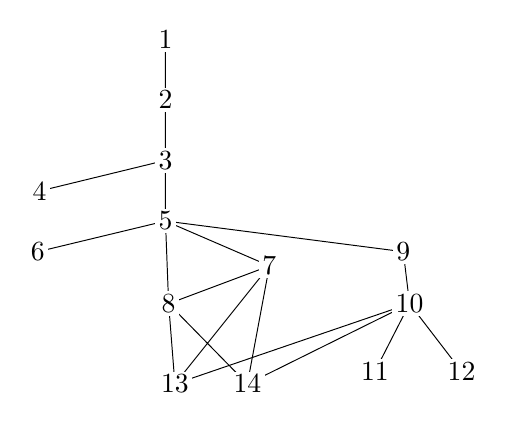
\begin{tikzpicture}[line width=0.35pt,every node/.style={fill=white,inner sep=1.2pt}]
  \coordinate (p1)  at ( 0.00, 0.00);
  \coordinate (p2)  at ( 0.00,-0.76);
  \coordinate (p3)  at ( 0.00,-1.53);
  \coordinate (p4)  at (-1.60,-1.92);
  \coordinate (p5)  at ( 0.00,-2.30);
  \coordinate (p6)  at (-1.62,-2.69);
  \coordinate (p7)  at ( 1.32,-2.87);
  \coordinate (p8)  at ( 0.04,-3.35);
  \coordinate (p9)  at ( 3.02,-2.69);
  \coordinate (p10) at ( 3.10,-3.35);
  \coordinate (p11) at ( 2.66,-4.21);
  \coordinate (p12) at ( 3.76,-4.21);
  \coordinate (p13) at ( 0.12,-4.37);
  \coordinate (p14) at ( 1.04,-4.37);
  \draw (p1)--(p2) (p2)--(p3) (p3)--(p4) (p3)--(p5)
        (p5)--(p6) (p5)--(p7) (p5)--(p8) (p5)--(p9)
        (p7)--(p8) (p7)--(p13) (p7)--(p14)
        (p8)--(p13) (p8)--(p14) (p9)--(p10)
        (p10)--(p11) (p10)--(p12) (p10)--(p13) (p10)--(p14);
  \node at (p1)  {1};  \node at (p2)  {2};
  \node at (p3)  {3};  \node at (p4)  {4};
  \node at (p5)  {5};  \node at (p6)  {6};
  \node at (p7)  {7};  \node at (p8)  {8};
  \node at (p9)  {9};  \node at (p10) {10};
  \node at (p11) {11}; \node at (p12) {12};
  \node at (p13) {13}; \node at (p14) {14};
\end{tikzpicture}
\end{center}
